\documentclass{standalone}
\usepackage{tikz}


\begin{document}

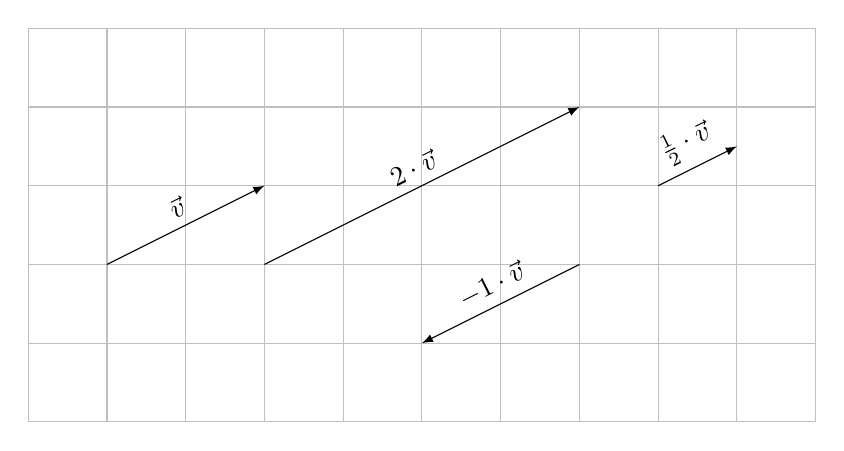
\begin{tikzpicture}
  \draw[thin,black!25] (0,0) grid (10,5);
  \draw[-latex] (1,2) -- ++(2,1) node[midway,sloped,above] {$\vec{v}$};
  \draw[-latex] (3,2) -- ++(4,2) node[midway,sloped,above] {$2 \cdot \vec{v}$};
  \draw[-latex] (7,2) -- ++(-2,-1) node[midway,sloped,above] {$-1 \cdot \vec{v}$};
  \draw[-latex] (8,3) -- ++(1,0.5) node[midway,sloped,above] {$\frac12 \cdot \vec{v}$};
\end{tikzpicture}

\end{document}